\documentclass{ecnreport}

\stud{OD Robotique 2016-2017}
\topic{Examen de Middleware/ROS - groupe B}

\begin{document}

\inserttitle{Examen de Middleware/ROS}

\insertsubtitle{1h, documents, codes de TP et internet autorisés}

\section{Travail demandé}

Le but de l'examen est de programmer Baxter pour qu'il détecte une couleur donnée et pointe un de ses bras vers l'objet détecté. Le tout se fera en simulation.
Le travail à rendre est sous la forme d'un fichier \texttt{main.cpp} (déjà existant et à modifier) et d'un fichier \texttt{control.launch} à créer.

\section{Initialisation de l'environnement}
  
\subsection{Si ROS n'est pas initialisé sur le compte}

Si votre environnement n'a pas encore été utilisé pour ROS, exécuter le script \texttt{ros\_user\_setup.sh} à télécharger depuis mon site web:
\defaultstyle
\begin{lstlisting}
wget http://pagesperso.ls2n.fr/~kermorgant-o/files/ros_user_setup.sh
sh ros_user_setup.sh
\end{lstlisting}
Refermez ensuite le terminal et ouvrez-en un nouveau.

\subsection{Téléchargement du package}

L'examen est téléchargeable sous forme de package ROS avec la commande suivante : 
\begin{center}\defaultstyle
\begin{lstlisting}
cd ~/ros/src
git clone https://github.com/oKermorgant/ecn_ros2016.git
\end{lstlisting}
\end{center}



\section{Description du package}

Le package téléchargé met en jeu 3 nodes qui communiquent via 4 topics. Le graphe est affiché ci-dessous.

\begin{figure}[h!]
 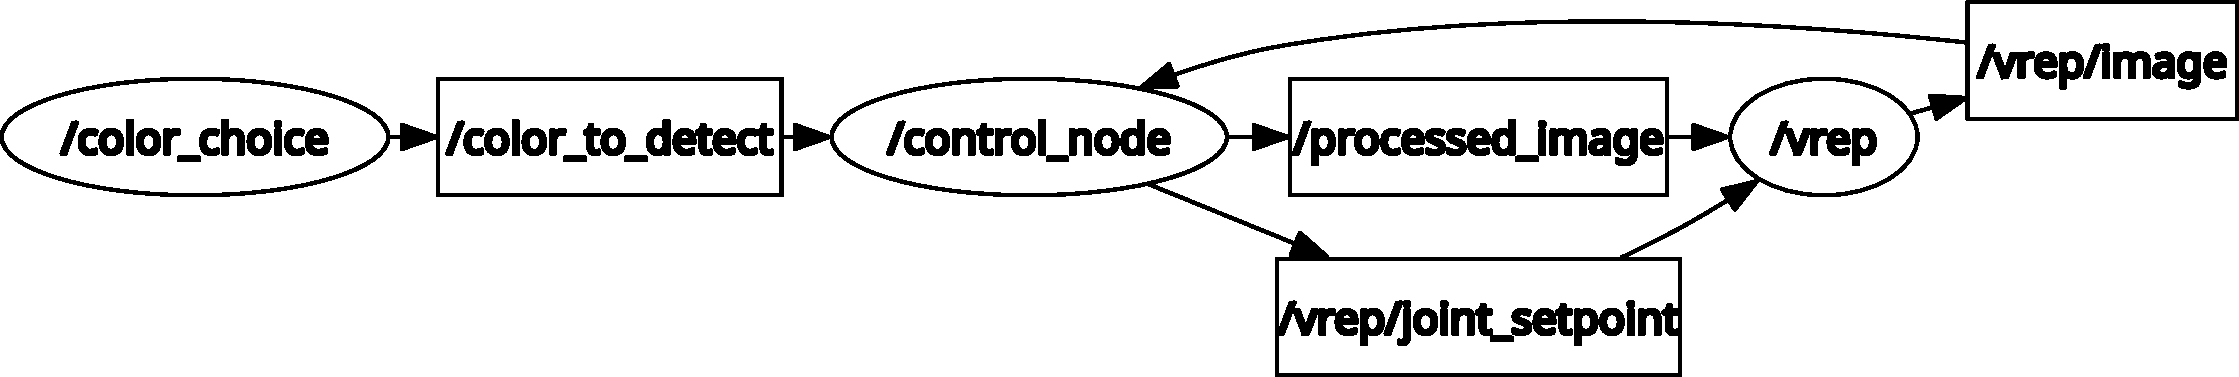
\includegraphics[width=\linewidth]{rosgraph}
 \caption{Graphe des nodes et topics}
\end{figure}


\subsection{Nodes et topics existants}

Lancez \texttt{vrep.launch}:
\begin{center}\defaultstyle
\begin{lstlisting}
roslaunch ecn_ros2016 vrep.launch
\end{lstlisting}
\end{center}

Le simulateur V-REP est lancé avec le robot Baxter se tenant devant une table comportant 4 objets de couleur. Il n'y a rien à faire dans l'interface du simulateur, 
tout passera par les topics. 
Le node principal est \texttt{/vrep} et correspond au simulateur. Ce node publie et souscrit à de nombreux topics et propose également de nombreux services. 
En pratique les services ne sont pas utilisés. 
Le node secondaire est \texttt{/color\_choice} et a pour fonction d'indiquer la couleur à détecter à chaque instant.\\
Les topics à considérer sont :
\begin{enumerate}
 \item \texttt{/vrep/image} : le simulateur y publie les images de la caméra de Baxter.
 \item \texttt{/vrep\_ros\_interface/joint\_command} : le simulateur y souscrit pour les consignes de position des bras de Baxter.
\item \texttt{/color\_to\_detect} : le node secondaire y publie la couleur à détecter.
 \end{enumerate}

\subsection{Paramètres}

Au lancement du simulateur, les valeurs RGB de plusieurs couleurs sont chargées en tant que paramètres ROS.
La valeur RGB d'une couleur est ainsi accessible via les paramètres :
\begin{center}
 $\left\{\begin{array}{lll}
\texttt{/colors/<couleur>/r} \\ \texttt{/colors/<couleur>/g} \\ \texttt{/colors/<couleur>/b}
         \end{array}\right.$
\end{center}

Par exemple, la syntaxe pour lire la valeur R de la couleur \texttt{blue} est ensuite :
\cppstyle
\begin{lstlisting}
std::string color = "blue";
int r;
nh.getParam("/colors/"+ color + "/r", r);
\end{lstlisting}

\section{Objectifs}


Le travail demandé est d'écrire :
\begin{itemize}
 \item Un node qui permet de détecter une couleur donnée (via un paramètre) et de publier la consigne de position correspondante.
 \item Un launchfile pour exécuter quatre fois le même node, détectant à chaque fois une couleur différente. Les couleurs à détecter sont : \texttt{blue, red, green, yellow}.
\end{itemize}
Il est fortement conseillé de développer une première mouture fonctionnelle du node en écrivant en dur la couleur qu'il détectera, avant de le rendre générique via le launchfile.\\
En bonus, le node peut également publier l'image traitée qui s'affichera dans V-REP. 


\subsection{Node à créer}

Un seul node est à créer en modifiant le fichier \texttt{main.cpp}. Ce fichier est compilé en un exécutable appelé \texttt{baxter\_color}. 
Le node devra :
\begin{itemize}
\item Lire les valeurs RGB correspondant à la couleur passée en paramètre.
\item Souscrire à \texttt{/vrep/image} pour avoir l'image courante. Ce topic contient des messages de type \texttt{sensor\_msgs/Image} qui peuvent être convertis en image OpenCV au sein du callback:
\cppstyle
\begin{lstlisting}
 im = cv_bridge::toCvCopy(msg, "bgr8")->image; 
\end{lstlisting}
\item Souscrire à \texttt{/color\_to\_detect} et la couleur courante à détecter. Ces messages sont de type \texttt{std\_msgs/String} dont la structure est :
\begin{lstlisting}
string data
\end{lstlisting} 
 \item Publier sur \texttt{/vrep\_ros\_interface/joint\_command} les consignes de position du bras. Ces messages doivent être de type \texttt{sensor\_msgs/JointState} dont la structure est:
\begin{lstlisting}
std_msgs/Header header
  uint32 seq
  time stamp
  string frame_id
string[] name
float64[] position
float64[] velocity
float64[] effort
 \end{lstlisting} où \texttt{name} contient les noms des articulations à contrôler et \texttt{position} contient les consignes de position des articulations. Les autres champs
 ne sont pas utilisés.
 \item Si la couleur à détecter est la couleur que le node doit détecter, traiter l'image et calculer la consigne de position des bras de Baxter.
 \item Si la couleur à détecter est la couleur que le node doit détecter, publier les consignes de position pour faire bouger le robot.
\end{itemize}

\subsection{Traitement d'image}

La partie détection de couleur est déjà implémentée dans une class appelée  \texttt{ColorDetector}. Cette classe est déjà instanciée mais les valeurs (r,g,b) doivent être 
récupérées via le paramètre ROS. La position en x et l'aire de l'object détecté sont obtenues via \texttt{cd.x()} et \texttt{cd.area()}.
Pour les objets considérés, une estimation de la position 3D est alors:
\begin{equation*}
  Z = \displaystyle \frac{0.106}{\sqrt{\text{area}}} \quad \text{et} \quad
        X = x.Z
\end{equation*}


\subsection{Consignes de position}

Seules 4 articulations sont à contrôler, dont les noms sont indiqués ci-dessous. 
Ces noms sont à renseigner dans le champ \texttt{name} du message de type \texttt{JointState}. \\
Les consignes sont à renseigner dans le champ \texttt{position} du message. Les valeurs des 4 consignes dépendent du signe de X, pour faire bouger un bras ou l'autre
en fonction de la position de l'objet détecté :
 \begin{center}
  \begin{tabular}{|C{6cm}|C{5cm}|C{5cm}|}\hline
   Articulation & Consigne si $X > 0$ & Consigne si $X < 0$ \\\hline
   \texttt{Baxter\_leftArm\_joint1} & $-\pi/4 + \text{atan2}(X-0.25,Z)$& $0$\\\hline
   \texttt{Baxter\_leftArm\_joint6} & $0$& $-\pi/2$\\\hline
   \texttt{Baxter\_rightArm\_joint1} & $0$& $\pi/4 - \text{atan2}(-X-0.25,Z)$\\\hline
   \texttt{Baxter\_rightArm\_joint6} & $-\pi/2$ & 0\\\hline
  \end{tabular}
 \end{center}
 


\subsection{Bonus}

Le node créé peut également publier l'image traitée après l'appel à la fonction \texttt{process}. Le topic sur lequel publier cette image est \texttt{/processed\_image}.
Le message doit être de type \texttt{sensor\_msgs/Image} qui peut être construit à la volée au moment de la publication avec :
\cppstyle
\begin{lstlisting}
cv::cvtColor(im_processed, im2, cv::COLOR_BGR2RGB);
im_pub.publish(cv_bridge::CvImage(std_msgs::Header(), "rgb8", im2).toImageMsg());
\end{lstlisting} 



\end{document}